\documentclass{article}
\usepackage[utf8]{inputenc}
\usepackage{listings}
\usepackage{color}
\usepackage{graphicx}
\usepackage{lscape}

\definecolor{dkgreen}{rgb}{0,0.6,0}
\definecolor{gray}{rgb}{0.5,0.5,0.5}
\definecolor{mauve}{rgb}{0.58,0,0.82}

\lstset{frame=tb,
  language=Java,
  aboveskip=3mm,
  belowskip=3mm,
  showstringspaces=false,
  columns=flexible,
  basicstyle={\small\ttfamily},
  numbers=none,
  numberstyle=\tiny\color{gray},
  keywordstyle=\color{blue},
  commentstyle=\color{dkgreen},
  stringstyle=\color{mauve},
  breaklines=true,
  breakatwhitespace=true,
  tabsize=3
}

\title{DM d'Architecture Logicielle}
\author{Sahin Tolga}
\date{3 May 2022}

\begin{document}

\maketitle

Ce document contiendra les diagrammes attendues par certaines questions.

\section{Q1/2 - Pattern Iterator}


\begin{figure}[!htb]
    \centering
    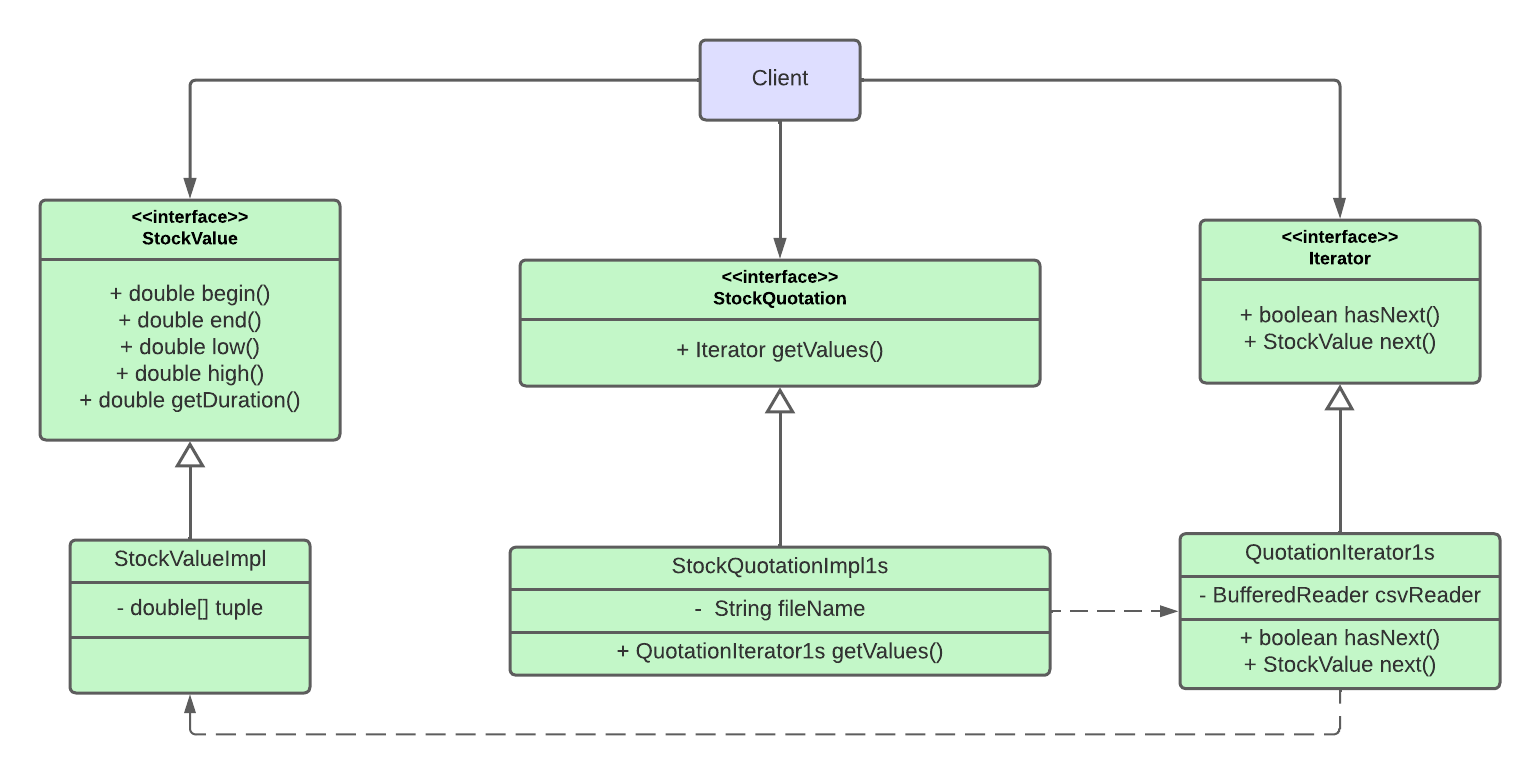
\includegraphics[width=14cm]{umls/iterator.png}
    \caption{Diagramme UML du Pattern Iterator}
    \label{fig:it1}
\end{figure}

\section{Q3 - Le code à trous}
\begin{lstlisting}
public class ex2020_21 {
    public static void main(String argv[]) {
        StockQuotation microsoft = new StockQuotationImpl1J("microsoft.csv");
        
        Iterator it = microsoft.getValues();

        int time = 0;

        while (it.hasNext()) {
            StockValue stockv = it.next();
            StringBuilder st = new StringBuilder();
            st.append(time);
            st.append(" , ");
            st.append(stockv.begin());
            st.append(" , ");
            st.append(stockv.end());
            st.append(" , ");
            st.append(stockv.low());
            st.append(" , ");
            st.append(stockv.high());
            System.out.println(st.toString());
            time += stockv.getDuration();
        }
        
    }
}

\end{lstlisting}

\section{Q5 - Pattern Decorator}

\begin{figure}[!htb]
    \centering
    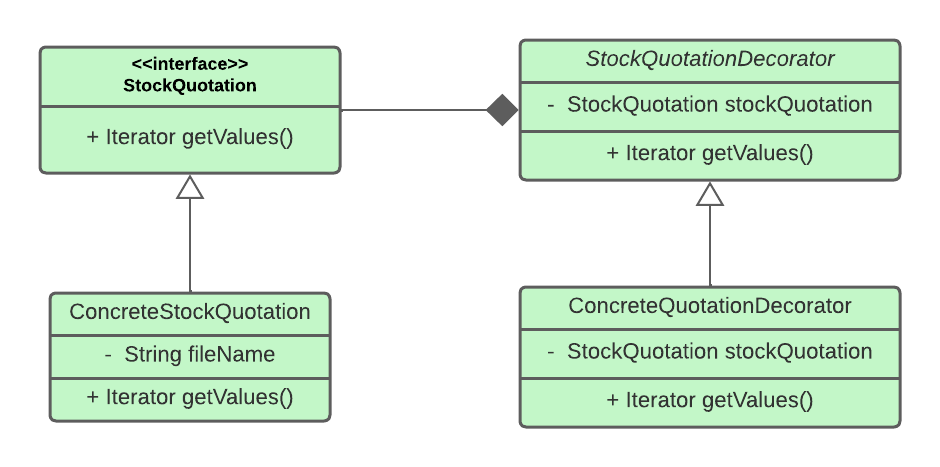
\includegraphics[width=14cm]{umls/decorator.png}
    \caption{Diagramme UML du Pattern Decorator}
    \label{fig:dec}
\end{figure}

\section{Q8 - Pattern Composite}

\begin{figure}[!htb]
    \centering
    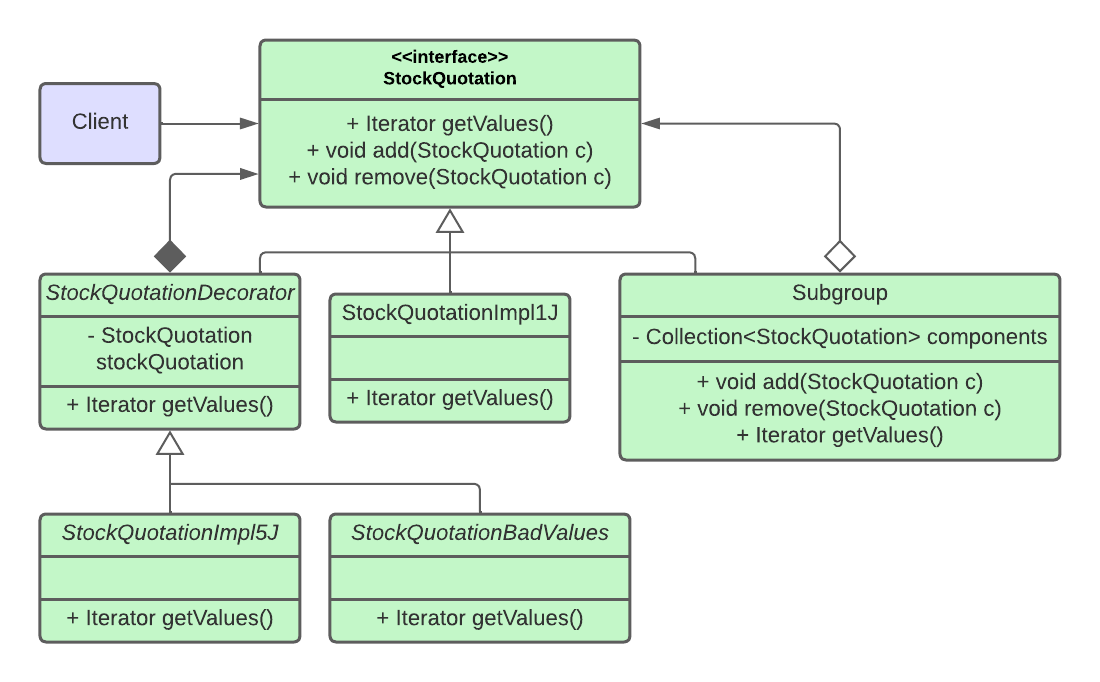
\includegraphics[width=10.5cm]{umls/comp.png}
    \caption{Diagramme UML du Pattern Composite}
    \label{fig:comp1}
\end{figure}

\section{Q9.1 - Architecture de la structure de groupe}

\begin{figure}[!htb]
    \centering
    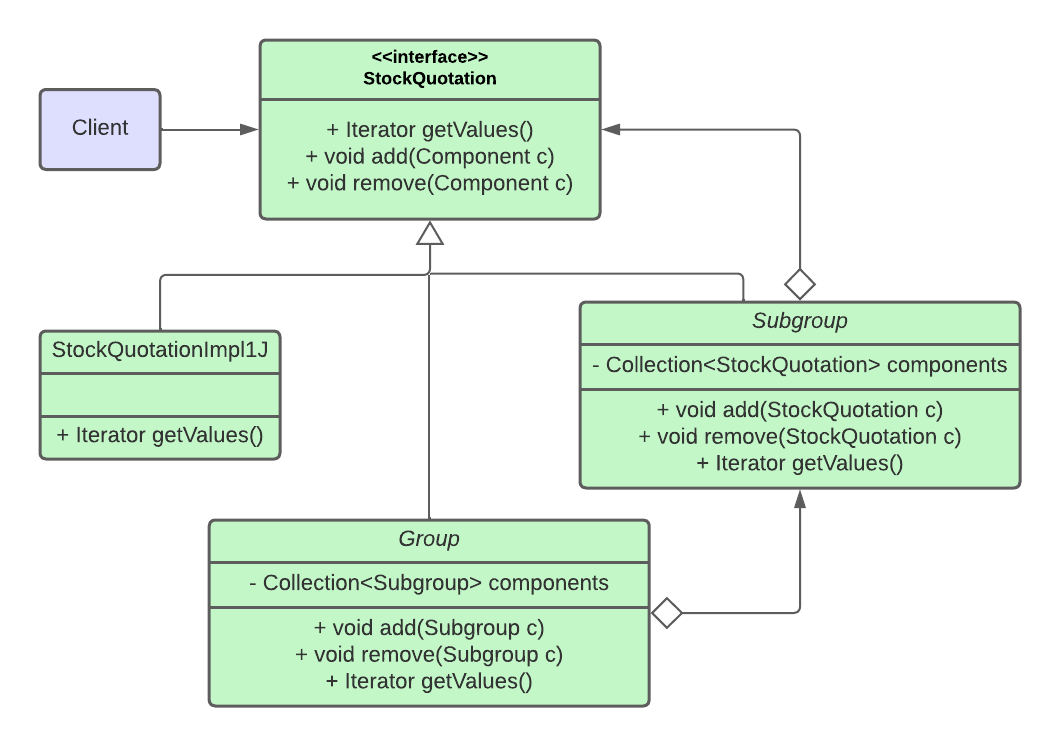
\includegraphics[width=10.5cm]{umls/compv2.png}
    \caption{Diagramme UML du Pattern Composite V2}
    \label{fig:comp2}
\end{figure}

\section{Q11 - Pattern Visitor}

\begin{figure}[!htb]
    \centering
    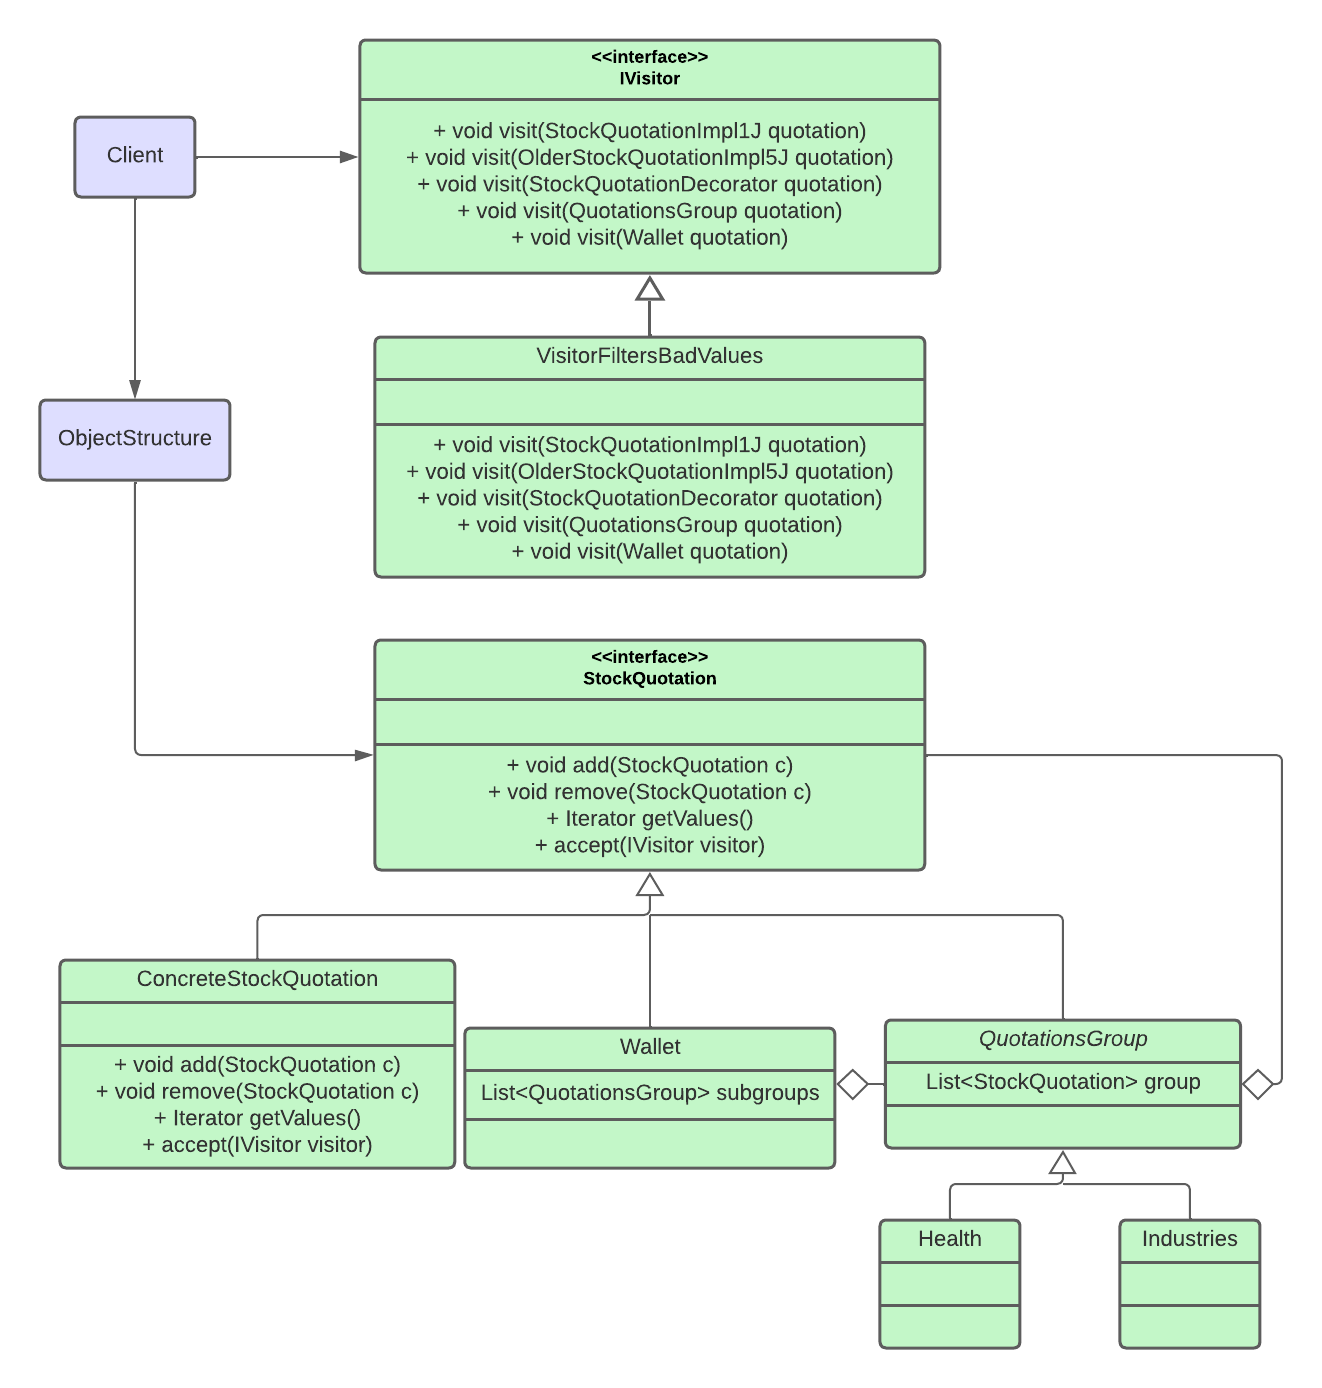
\includegraphics[width=11cm]{umls/visitor.png}
    \caption{Diagramme UML du Pattern Visitor}
    \label{fig:vis1}
\end{figure}

\section{Architecture du projet}

Vous trouverez dans le fichier "project.png", un UML généré de mon projet. Je n'y ai pas ajouté tous les liens d'associations pour simplifier la lisibilité, de toute manière cela suit les mêmes idées schématisées auparavant.


\end{document}
